\documentclass{article}
\usepackage{float}
\usepackage{graphicx} % Required for inserting images
\usepackage[hidelinks]{hyperref} % Required for using links

%Allow to use pdf images
\usepackage{pdfpages}

%Packages and instruction to change scale of sections', subsections' and subsubsections' heads
\usepackage{titlesec}
\usepackage{titlesec}
\titleformat*{\section}{\Huge\bfseries}
\titleformat*{\subsection}{\LARGE\bfseries}
\titleformat*{\subsubsection}{\Large\bfseries}

%Instruction used to create a new subsection level (subsubsubsection) in the document
\titleclass{\subsubsubsection}{straight}[\subsection]
%Instructions used to create a new counter for the subsubsubsections and create the command to invoke(use) them
\newcounter{subsubsubsection}[subsubsection]
\renewcommand\thesubsubsubsection{\thesubsubsection.\arabic{subsubsubsection}}

%Instruction used to align the new section layer in a correct manner in the table of contents
\makeatletter

%Instructions to change the scale and font of the subsubsubsections' head
\titleformat{\subsubsubsection}
  {\normalfont\large\bfseries}{\thesubsubsubsection}{1em}{}
\titlespacing*{\subsubsubsection}
{0pt}{3.25ex plus 1ex minus .2ex}{1.5ex plus .2ex}

%Instructions to create the subsubsubsections entries in the table of contents (included the dot line)
\def\toclevel@subsubsubsection{4}
\def\l@subsubsubsection{\@dottedtocline{4}{7em}{4em}}

%Instruction used to make link to part of the document using table of contents
\makeatother

%Instructions to set table of contents and sections depth to 4 layers
\setcounter{secnumdepth}{4}
\setcounter{tocdepth}{4}

%Used in order to have more symbols for itemize lists
\usepackage{pifont}

%Used to make the header and footer of each document page
\usepackage{fancyhdr}

%Defines a new style of header and footer
\fancypagestyle{IntroductionStyle}{
\fancyhf{}
\fancyhead[L]{\textit{\textbf{SECTION 1. INTRODUCTION}}}
\fancyfoot[L]{CKB \quad - \quad \textbf{R}equirements \textbf{A}nalysis \textbf{S}pecifications \textbf{D}ocument}
\rfoot{\thepage}
\renewcommand{\headrulewidth}{0.4pt}
\renewcommand{\footrulewidth}{0.4pt}
}
\fancypagestyle{OverallDescriptionStyle}{
\fancyhf{}
\fancyhead[L]{\textit{\textbf{SECTION 2. OVERALL DESCRIPTION}}}
\fancyfoot[L]{CKB \quad - \quad \textbf{R}equirements \textbf{A}nalysis \textbf{S}pecifications \textbf{D}ocument}
\rfoot{\thepage}
\renewcommand{\headrulewidth}{0.4pt}
\renewcommand{\footrulewidth}{0.4pt}
}
\fancypagestyle{SpecificRequirementsStyle}{
\fancyhf{}
\fancyhead[L]{\textit{\textbf{SECTION 3. SPECIFIC REQUIREMENTS}}}
\fancyfoot[L]{CKB \quad - \quad \textbf{R}equirements \textbf{A}nalysis \textbf{S}pecifications \textbf{D}ocument}
\rfoot{\thepage}
\renewcommand{\headrulewidth}{0.4pt}
\renewcommand{\footrulewidth}{0.4pt}
}
\fancypagestyle{FormalAnalysisAlloyStyle}{
\fancyhf{}
\fancyhead[L]{\textit{\textbf{SECTION 4. FORMAL ANALYSIS USING ALLOY}}}
\fancyfoot[L]{CKB \quad - \quad \textbf{R}equirements \textbf{A}nalysis \textbf{S}pecifications \textbf{D}ocument}
\rfoot{\thepage}
\renewcommand{\headrulewidth}{0.4pt}
\renewcommand{\footrulewidth}{0.4pt}
}
\fancypagestyle{EffortSpentStyle}{
\fancyhf{}
\fancyhead[L]{\textit{\textbf{SECTION 5. EFFORT}}}
\fancyfoot[L]{CKB \quad - \quad \textbf{R}equirements \textbf{A}nalysis \textbf{S}pecifications \textbf{D}ocument}
\rfoot{\thepage}
\renewcommand{\headrulewidth}{0.4pt}
\renewcommand{\footrulewidth}{0.4pt}
}

%Used to handle table width and split tables across different pages
\usepackage{xltabular}
%Change space between table columns
\setlength{\tabcolsep}{18pt}

%Command used to create a new column type whose background is lightgray colored
\usepackage{xcolor,colortbl}
\definecolor{LightGray}{gray}{0.85}
\newcolumntype{g}{>{\columncolor{LightGray}}c}


%Set the default path of images
\graphicspath{ {images/} }

\title{RASD-v0.5}
\author{Francesco Spangaro - Tosetti Luca - Francesco Riccardi}
\date{October 2023}

\begin{document}

\maketitle

\begin{figure}[h]
    \centering
    
\includegraphics[scale=0.5]{politecnico-di-milano-logo.png}
\end{figure}



\tableofcontents

\newpage

\pagestyle{IntroductionStyle}

\section{Introduction}
    \subsection{Purpose}
        The purpose of the CodeKataBattle platform is to create a friendly and enjoyable environment for students
        to acquire new skills and improve the ones already owned in Software Development. This is done by allowing students to train and compete with each others by writing code in order to resolve problems. All of this under the supervision of educators who can challenge their students to take part to these competitions.
        \subsubsection{Goals}
            \begin{description}
                %Educator's goals
                \item[G1:] \textit{\textbf{Allow educators to create new tournaments:}}
                    \begin{description}
                        \item Educators have the possibility to create new tournaments. 
                            When creating a tournament, educators have the opportunity to create new badges. Badges have corresponding achievements, called "Rules", which are defined on badge creation. Badges are obtained by users on achievement completion. Obtained badges will be then displayed on the user's profile page.
                    \end{description}
                \item[G2:] \textit{\textbf{Allow educators to create new battles:}}
                    \begin{description}
                        \item Educators have the possibility to define new battles within tournament they crated or in tournaments      they have been granted permission to do so. When creating a new battle educators have to set different         parameters:
                        \begin{itemize}
                            \item upload project description;
                            \item specify the programming language and build tool to utilize, including test cases and build automation scripts;
                            \item set minimum and maximum number of students per group;
                            \item set a registration deadline;
                            \item set a final submission deadline;
                            \item set additional configuration for scoring.
                        \end{itemize}
                    \end{description}
                    % Assumption: educators can access al tournaments and battles with view only permission
                \item[G3:] \textit{\textbf{Allow educators to administer different tournaments:}}
                    \begin{description}
                        \item Educators can grant other colleagues permission to create new battles in their tournaments. Educators have the possibility to close their tournaments, thus, not letting students submit new answers to any battle defined in the closed tournament, nor letting their colleagues create new battles in that tournament. 
                    \end{description}
                    % Ask if rank visualization is a goal or a user-interface point 
                \item[G4:] \textit{\textbf{Allow educators to administer different battles:}}
                    \begin{description}
                        \item Educators have the possibility, once a battle has expired, to manually evaluate through the platform each student's work, and then assign a corresponding score to each one of them, ranging from 0 to 100. 
                    \end{description}
                %Students' goals
                \item[G5:] \textbf{\textit{Allow students to subscribe in tournaments:}}
                    \begin{description}
                        \item Students subscribed to the platform have the possibility to subscribe to different tournaments, in which they plan to participate in.
                    \end{description}
                    % Assumption: to do anything, both students and educators must be already subscribed to the platform 
                \item[G6:] \textbf{\textit{Allow students to participate in battles:}}
                    \begin{description}
                        \item Students can join battles within a set deadline. They can do so by themselves, by inviting somebody else or by accepting someone's else invite.
                        \begin{description}
                            \item[G6.1:] \textbf{\textit{Allow students to form groups to participate with:}}
                                \begin{description}
                                    \item Students have the possibility to send out invitations to other students, so that they can form a group to participate with. Groups need to follow the guidelines specified by the battle creator for it to be accepted.
                                \end{description}
                            \item[G6.2:] \textit{\textbf{Allow students to submit their answers:}}
                                \begin{description}
                                    \item When students have developed a solution to the battle, they can submit their answer to the platform. Groups are requested to send only one answer. Students can change their answer as they proceed, when uploading a new solution the older one is overwritten, since there can only be one answer for each battle. 
                                \end{description}
                            \item[G6.3:] \textit{\textbf{Allow students to see their scores:}}
                                \begin{description}
                                    \item After each answer submission, a new score is assigned to the students. The score can be manually created by an educator or automatically assigned to the students by the platform. Students can see the scores obtained
                                \end{description}
                        %TODO
                        % Ask professor if score is computated each commit, not visualized, and then published after battle closing, or if students can actively see their scores as the battle progresses (par. 2, last line - par. 4, last line) 
                        \end{description}
                    \end{description}
                \item[G7:] \textit{\textbf{Let the students be notified on important events:}}
                    \begin{description}
                        \item When a new tournament is created, all students subscribed to the platform are notified. A different notification will be sent when a new battle is created in a tournament they are subscribed to.
                        % ask if this goal is correct
                    \end{description}
            \end{description}
\subsection{Scope}
    CodeKataBattle (CKB) is an easy-to-use platform, which aims to allow educators to propose homework and/or lessons in a new and fresh way to involve students more in acquiring and improving software developing skills. To do that, CKB offers educators the possibility to open several tournaments. Each tournament is composed by several battles in which students can compete with each other, individually or in groups. 
    In order to offer all of this CKB relies on the external platform GitHub. GitHub will take the role of a "bridge" between CKB platform and students, allowing them to upload their solutions on it. These solutions will be then taken by the CKB platform from GitHub and used to evaluate student's score in the battle for which they uploaded a specific solution. 
\subsubsection{Phenomena}
    Events that take place either in the real world, in machine world or in both. Used to describe respectively what cannot be observed by the machine, real world and event that connects the two.
    \subsubsubsection{World phenomena}
        Phenomena events that take place in the real world and are not observable by the machine
        \begin{enumerate}
            \item[\textbf{WP1:}] Students fork the GitHub repository of which they received a link by the platform.
            \item[\textbf{WP2:}] Student write code on his personal device.
            \item[\textbf{WP3:}] Students choose which tournament to join
            \item[\textbf{WP4:}] Students choose which battle to join in a tournament precedently joined.
            \item[\textbf{WP5:}] Student choose his teammates for a battle.
            \item[\textbf{WP6:}] Educator choose whether and which colleagues to allow access to one of his tournaments
            \item[\textbf{WP7:}] Student subscribed to a battle wait for its start (registration deadline expiration)
            \item[\textbf{WP8:}] Educator decide to close a tournament
        \end{enumerate}

    \subsubsubsection{Shared phenomena}
        \begin{itemize}
            \item Phenomena controlled by the world and observed by the machine
            \begin{enumerate}
                \item[\ding{228}] Student related phenomena 
                \begin{enumerate}
                    \item[\textbf{SP1:}] Student registration to the platform
                    \item[\textbf{SP2:}] Student log in to the platform
                    \item[\textbf{SP3:}] Student subscribe to a tournament within a deadline
                    \item[\textbf{SP4:}] Student invite other students to form a team
                    \item[\textbf{SP5:}] Student accept an invite from another student and join its group.
                    \item[\textbf{SP6:}] Student or a group of students join a battle in a tournament they are subscribed to within a deadline.
                    \item[\textbf{SP7:}] Student upload a new software solution for the battle's problem, in which he's partecipating
                    \item[\textbf{SP8:}] Student sees its, and others badges visualizing its or others profile page
                    \item[\textbf{SP9:}] Student or a group of it, push a new commit on GitHub repository
                \end{enumerate}
                \item[\ding{228}] Educator related phenomena
                \begin{enumerate}
                    \item[\textbf{SP10}:] Educator create a new tournament
                    \item[\textbf{SP11}:] Educator grant access to his other collegues to create new battle within a tournament he created
                    \item[\textbf{SP12}:] Educator create a new battle
                    \item[\textbf{SP13}:] Educator set battle's setting while creating one of them
                    \item[\textbf{SP14}:] Educator manually evaluate the work done by students in a certain battle of a certain tournament during battle's consolidation phase
                    \item[\textbf{SP15}:] Educator closes a tournament
                    \item[\textbf{SP16}:] Educator defines new badges achievable in a tournament by students while creating it
                    \item[\textbf{SP17}:] Educator sees collected badges of a student by visualizing its profile page
                \end{enumerate}
            \end{enumerate} 

            \item Phenomena controlled by the machine and observed by the World.
            \begin{enumerate}
                \item[\ding{228}] Student related phenomena
                \begin{enumerate}
                    \item[\textbf{SP18}:] Student registered to the platform gets notified when a new tournament is created
                    \item[\textbf{SP19}:] Student subscribed to a tournament gets notified of upcoming battle created in that tournament
                    \item[\textbf{SP20}:] Student receive from the platform a invite notification in order to join a group of students to join a battle.
                    \item[\textbf{SP21}:] Platform, when a battle's registration deadline expires, send every student that joined the battle a link to the GitHub repository created by the platform itself.
                    \item[\textbf{SP22}:] Platform at the end of each battle updates students' score in the tournament in which battle took place allowing all students and educators to see them
                    \item[\textbf{SP23}:] Students get notified when a tournament is closed
                \end{enumerate}
                \item[\ding{228}] Educator related phenomena
                \begin{enumerate}
                    \item[\textbf{SP24}:] Educator receive a notification when allowed by a collegue to access its collegue's tournament.
                    \item[\textbf{SP25}:] Educator gets notified when submission deadline of solution for a battle expires, and start the consolidation phase.
                \end{enumerate}
            \end{enumerate}
        \end{itemize}

    \subsubsubsection{Machine phenomena}
        Phenomena events that take place in the machine world and are not observable from the real world
        \begin{enumerate}
            \item[\textbf{MP1:}] The platform creates a GitHub repository containing the code kata when registration deadline of a battle expires.
            \item[\textbf{MP2:}] The platform when notified by GitHub API pulls the latest sources of the repository of a battle
            \item[\textbf{MP3:}] The platform analyzes the sources, by running tests on them.
            \item[\textbf{MP4:}] The platform calculate the battle score of a team based on the executables uploaded by students for a battle. Score is automatically updated when the platform receive notification from GitHub about new push actions.
            \item[\textbf{MP5:}] The platform at the end of each battle of a tournament, compute the tournament rank of each student in that tournament.
            \item[\textbf{MP6:}] The platform automatically register badges acquirement from a student, when that student satisfy the rules to obtain them.
        \end{enumerate}

    
\subsection{Definitions, acronyms, abbreviations}
    \subsubsection{Definitions}
        {\renewcommand{\arraystretch}{1.5}
            %\textwidth used to set table's width according to text's width of the page
            %">{\raggedright\arraybackslash} c" used to align to the right the column c
            %"X" column tag creates a paragraph-like column whose width automatically expands so that the declared width of the environment is filled
            \begin{xltabular}{\textwidth}{ >{\raggedright\arraybackslash}c >{\raggedright\arraybackslash}X }
                \hline 
                \textbf{Term} & \textbf{Definition} \\
                \hline 
                
                \endfirsthead   %Everything above is used as "head" (first row) of
                                %the table in the page where it is placed

                \hline 
                \textbf{Term} & \textbf{Definition} \\
                \hline 

                \endhead    %Everything above is used as "head" (first row) of the
                            %splitted parts of the table in the pages different from
                            %the one in which the table was originally placed
                
                \endfoot    %Everything above is used as "foot" (last row) of the
                            %splitted parts of the table in the pages different from
                            %the last one in which the table appear

                \endlastfoot    %Everything above is used as "foot" (last row) of the
                                %table in the page where it appears last.
    
                \textit{GitHub Repository} & $\rightarrow$ A place on the GitHub platform where a user can store code, files and each file's revision history. \\
                \textit{Registration deadline} & $\rightarrow$ Maximum time within which a student can subscribe to a battle or to a tournament. \\
                \textit{Submission deadline} & $\rightarrow$ Maximum time within which a student, or a group of student, can upload their solution to a battle problem \\
                \textit{Code Kata} & $\rightarrow$ The word kata refers to a karate exercise in which a form gets repeated many time, making little improvements in each tentative.
                In this context it's used to express the fact that the code need to be developed multiple times to reach a optimal solution to the battle problem. \\
                \textit{Consolidation phase} & $\rightarrow$ Phase started at the end of a battle, used to consolidate the score of each student in the battle by eventually a manual evaluation of the students' code by an Educator. \\
                \textit{View-only mode} & $\rightarrow$ An abstract modality (not an implementation detail) in which educator can be if he access to a tournament in which they have no rights to create new battles \\
                \textit{Modify-enabled mode }& $\rightarrow$ An abstract modality (not an implementation detail) in which educator can be if he access to a tournament in which he go granted the access by tournament's creator, and thus can create new battles.
            \end{xltabular}
    
        % \textit{GitHub Repository} $\rightarrow$ A place on the GitHub platform where a user can store code, files and each file's revision history.
        % \\ \\
        % \textit{Registration deadline} $\rightarrow$ Maximum time within which a student can subscribe to a battle or to a tournament.
        % \\ \\
        % \textit{Submission deadline} $\rightarrow$ Maximum time within which a student, or a group of student, can upload their solution to a battle problem
        % \\ \\
        % \textit{Code Kata} $\rightarrow$ The word kata refers to a karate exercise in which a form gets repeated many time, making little improvements in each tentative.
        % In this context it's used to express the fact that the code need to be developed multiple times to reach a optimal solution to the battle problem.
        % \\ \\
        % \textit{Consolidation phase} $\rightarrow$ Phase started at the end of a battle, used to consolidate the score of each student in the battle by eventually a manual evaluation of the students' code by an Educator.
        % \\ \\
        % \textit{View-only mode} $\rightarrow$ An abstract modality (not an implementation detail) in which educator can be if he access to a tournament in which they have no rights to create new battles
        % \\ \\
        % \textit{Modify-enabled mode} $\rightarrow$ An abstract modality (not an implementation detail) in which educator can be if he access to a tournament in which he go granted the access by tournament's creator, and thus can create new battles.
        

    \subsubsection{Acronyms}
        \begin{xltabular}{\textwidth}{ >{\raggedright\arraybackslash}c >{\raggedright\arraybackslash}X }
            \hline 
            \textbf{Acronym} & \textbf{Meaning} \\
            \hline 
                
            \endfirsthead

            \hline 
            \textbf{Acronym} & \textbf{Meaning} \\
            \hline 

            \endhead
            \endfoot
            \endlastfoot

            \textit{API} & $\rightarrow$ Application Programming Interface, indicates on demand procedure which supply a specific task
            \\
            \textit{CKB} & $\rightarrow$ CodeKataBattle, the name of the platform described in this document
            \\
            \textit{IT} & $\rightarrow$ Used as acronym for Information Technology which identify something, generally a computing or communication hardware, with information storage capability and closely related to the informatic world.
            \\
            \textit{UML} & $\rightarrow$ Unified Modeling Language, a standard notation for modeling real world object, in an high level diagram representing OO components.
            \\
            \textit{BPMN} & $\rightarrow$ Stands for Business Process Modeling Notation, standard notation to represent processes through diagrams.  
            \\
            \textit{OO} & $\rightarrow$ Object-Oriented is a programming paradigm based on the concept of object which can contain data and code, and represent usually real world object.
            
        \end{xltabular}
        
        % \textit{API} $\rightarrow$ Application Programming Interface, indicates on demand procedure which supply a specific task
        % \\ \\
        % \textit{CKB} $\rightarrow$ CodeKataBattle, the name of the platform described in this document
        % \\ \\
        % \textit{IT} $\rightarrow$ Used as acronym for Information Technology which identify something, generally a computing or communication hardware, with information storage capability and closely related to the informatic world.
    \subsubsection{Abbreviations}
       \begin{xltabular}{\textwidth}{ >{\raggedright\arraybackslash}c >{\raggedright\arraybackslash}X }
            \hline 
            \textbf{Abbreviation} & \textbf{Meaning} \\
            \hline 
                
            \endfirsthead

            \hline 
            \textbf{Abbreviation} & \textbf{Meaning} \\
            \hline 

            \endhead
            \endfoot
            \endlastfoot

            \textit{G\#} & $\rightarrow$ Goal number \#
            \\
            \textit{WP\#} & $\rightarrow$ World phenomena number \#
            \\
            \textit{SP\#} & $\rightarrow$ Shared phenomena number \#
            \\
            \textit{MP\#} & $\rightarrow$ Machine phenomena number \#
            \\
            \textit{D\#} & $\rightarrow$ Domain assumption number \#
            \\
            \textit{c.s.} & $\rightarrow$ Computer science
            \\
            \textit{e.g.} & $\rightarrow$ Exempli gratia, latin phrase corresponding to "for example"
        \end{xltabular}     

\subsection{Revision history}
    \begin{itemize}
        \item **Placeholder data**: version 1.0
        \item **Placeholder data**: version 1.1
        \item **Placeholder data**: version 1.2
        \item **Placeholder data**: version 2.0
        \item **Placeholder data**: version 2.1
    \end{itemize}    
\subsection{Reference documents}
    GitHub references:
    \begin{itemize}
        \item Official documentation to get started with GitHub: $\rightarrow$ \url{https://docs.github.com/en/get-started/quickstart}
        \item Official documentation about fork process $\rightarrow$ \url{https://docs.github.com/en/get-started/quickstart/fork-a-repo}
        \item Official documentation about GitHub actions $\rightarrow$ \url{https://docs.github.com/en/actions}
    \end{itemize}
    UML official specification $\rightarrow$ \url{https://www.omg.org/spec/UML}
    \\ \\
    BPMN official specification $\rightarrow$ \url{https://www.omg.org/spec/BPMN/2.0}
\subsection{Document structure}
    \begin{itemize}
        \item \textbf{\textit{Section 1: Introduction}} \\
        This section introduces the problem and the platform/application to be developed in order to resolve it. It describes the major purpose of the project, every one of his goals, the analysis of the its domain and every world, shared and machine phenomena associated with it.
        In addition in this section are inserted the definitions, acronysm and abbreviations used in this ddocument, including even it's revision history and refereced documents or web pages.
        \item \textbf{\textit{Section 2: Overall description}} \\
        This section gives an overall description of the project and all the interactions that could occur between the platform and the final users (Students and educators). To do this, it will include different possibile scenarios that could happen, the different actors involved in the platform usage and all the assumptions, dependencies and eventual constraints that have to be considered in the development of the platform
        \item \textbf{\textit{Section 3: Specific Requirements}} \\
        This section is the most technical one, it contains more precise descriptions of each scenario called use cases. It describe the several functional and performance requirements of the project and their map to the goals of the project.
        Finally it contains also all the design constraint and system attributes that must be followed/guaranteeded while developing the platform.
        \item \textbf{\textit{Section 4: Formal analysis using allo}}y \\
        In this setion can be found a formal description of the platform/application. The formal description is done using the formal language Alloy (referenced in section 1)
        \item \textbf{\textit{Section 5: Effor spent}} \\
        A simple section in which are included all the information about the time requested by each group member to complete this document, and it's division by each section of the document.
    \end{itemize}

\newpage

\pagestyle{OverallDescriptionStyle}

\section{Overall description}
    \subsection{Product perspective}
        The following section contains the UML diagram of the platform and a list of meaningful scenarios in which the platform can be used, how and when users can interact with it.
        \subsubsection{Scenarios}
            \subsubsubsection{Student sign up to the platform}
                Peter is a volenterous student of an informatic class, that want to improve his software development skills. He comes to know about the platform CKB one day, when his c.s. professor propose to his class, a software development tournament in substitution to the normal, boring and limited tests organized through the academic year.
                Peter is extremely interested, not only in the tournament, but also in the service offered by the platform itself, thus the same day he decide to try to register to it.
                Peter open his personal browser and go to the CKB site's homepage. Here he goes to the student dedicated page and clicks the "Sign up" button in order to register. He inserts all the required information in the mandatory fields of the page that showed up (e.g. name, surname, attended school, email, username, password, ...) and clicks on "Confirm" button.
                Peter now wait for the notification, through his email, about the correctness of his registration, and can now access all the CBK platform's features after loggin in with it's credentials.
            \subsubsubsection{Educator sign up to the platform}
                Vittorio is an innovative teacher who teaches c.s. in a school. He discovered, while searching the web for new ideas on how testing his students' abilities in software developing, the CKB platform and its services.
                Vittorio decide to try to register to the platform, as he's very intrigued about it. To do that Vittorio goes on the CKB Homepage and then on the page dedicated to educators and clicks the "Sign up" button. At this point he compiles all the fields in the form that showed up with the new page (e.g. name, surname, school in which he teaches, istitutional email, password, ...), especially the fields related to his profession, and in the end clicks on "Confirm" button.
                Finally Vittorio wait for the registration confirm email, and start using CKB platform's features after loggin in with it's credentials.
            \subsubsubsection{Educator creates a new tournament (and badges)}
                Laura is an c.s. educator who registered to CKB platform. She decide to create a new tournament to let her student compete with each other and improve their software developing skills. In order to do so, Laura log in her account on the platform and try to create a new tournament. While doing so, she decide which programming languages can be used to develop the solution to the battles that will be contained in the tournament, the name of the tournament, the method through which students can access it, eventually its maximum duration, and finally she decide if the tournament will contains some new or default badges, obtainable by the students by doing some achievements.
                Laura wants to create new particular badges, in order to encourage her students to participate more actively to the tournament. To do so, Laura access the appopriate section during tournament creations, and starts creating the badges, specifing their title, rules to obtain them, their icon and eventually their score, that will be added to the student's score that obtained them.
                At the end of the process Laura, confirm her choices and the tournament starts.
            \subsubsubsection{Educator creates a new battle}
                Laura is an c.s educator who registered to the CKB platform. After she created a new tournament, Laura wants to immediately create a new battle within it, to let her students compete with each other. To do so Laura, log in her account on the platform, access the tournament in which she wants to create a new battle through an appropriate web page. At this point Laura try to create a new battle within the tournament. While doing so, she decide the battle's name, the programming language allowed in the battle, maximum number of partecipant, dimension of group of students that can partecipate to it, a registration and submission deadline and eventually sets some personalized rules to calculate students' score in the battle.
                At the end of all of this process, Laura waits for the students of her class, subscribed to the tournament in which the battle has been created, to join the battle. At the end of the registration deadline, partecipant can start competing with each other, while Laura can supervise their work.
                At the end of the battle, which automaticcaly close itself at submission deadline, students' score gets calculated and added to their tournament score.
            \subsubsubsection{Educator close a tournament}
                Marco is an c.s educator who registered to the CKB platform. He has created a new tournament one mounth ago, today, after this mounth he decide to close it. In order to do so, Marco log in his account on the platform and access the tournament which he wants to close through an appropriate web page, at this point Marco control il there are battles that aren't altready closed and sees that Laura has a tournament that is still open, so he now control when is the submission deadline of this battle. After discovering that the submission deadline is in two days he close the possibility of other educators to creates new battles.
                After three days Marco, after log in to the platform, control that there are'n still open tournament or tournament that are waiting for the manual evaluation. Then he proceed to close the tournament
            \subsubsubsection{Educator manually evaluate a battle after the end}
                Luca is an c.s educator who registered to the CKB platform. He has created a new battle in a tournament two weeks ago, choosing as the submission deadline yesterday and choosing to include a Manual evaluation in the total evaluation of the battle, according to the requirments of shared balaced partecipation, optimization and writing comments related to the code and the implementative choice.
                Today, Luca log in his account on the platform, access to the tournament in which he created the battle and see that this battle in closed and is waiting for a manual evaluation and decide to examine the codes that have been delivered in the battle by the different groups.
                The first group he analyzes is made un of three students, and sees that they have a score of 90/100 in the automated evaluation. After entering on the resource made available by the group, Luca check if the number of commits and work ha ìs been done equally among the students in the group and not noticing large differences between the number of lines of code written and the number of commit made by each student he decide to go next to the comment section.
                Opening the code in the resource, he relizes that the group has limited himself to adding simple comments, without going to much in the details of the work done and choices made; so he decide to modify the grade assigned befor, by reducing it from 90/100 to 80/100, writing a little explanation of the reason for this change. It then continues to control all the others group and at the end he can close formally the battle.
            \subsubsubsection{Student forms a group then joins a battle}
                Francesca singns in the platform with her credentials and sees that a new tournament has opened. Shoe would like to participate in it, and so decides to form a group with two of her friends to compete in the tournament's battles. She clicks on the apposite menu and chooses the users she would like to invite to join her group.
                After both her friends accept her invite, she enters the tournament by signing up her group as participant. She then looks at all of the proposed battles they can join in, and chooses one.
                Once the registration deadline for the groups expires, Francesca's group forks the automatically created GitHub repository and sets up an automated workflow through GitHub Actions, to notify the platform of each of their commits.
            \subsubsubsection{Student uploads a solution}
                Piero is currently competing with his group in a tournament, they are working on a solution for a battle and they are confident that they are right with what they coded. Piero decides to upload a solution for the battle to the GitHub repository, so that it can be evaluated and they can see how much their score is for this first draft solution.
                Piero uploads the current solution to the forked GitHub repository. After the push, the GitHub Actions workflow is started, letting the platform know that Piero has uploaded a new solution for the battle he's currently competing in.
                The automated evaluation system integrated in the platform now starts, tests are automatically ran and no human evaluation is deemed needed, so the platform gives Piero's solution a score of 75/100.
                Piero sees the score on his profile on the platform and understands that his solution is found correct, but not the best that can possibly be done. He decides to continue working on it, until his solution will obtain a score of at least 95/100.
            \subsubsubsection{Student uploads a solution after deadline expiration time}
                Frank has been competing in a tournament for very long, and has finally found a solution for the last battle he struggled to solve. After having uploaded his solution on the forked repository, the GitHub Actions workflow starts and notifies the platform that Frank's has uploaded a new solution for his final battle.
                The CodeKataBattle platform then sees that the deadline for Frank's battle has expired. The platform notifies Frank that his last uploaded solution will not be considered on the final score he will get, and no further action is taken.
            \subsubsubsection{Students visualize his tournament's results and his badges}
                Paolo, Lucia e Alessandro are three friends that are subscribed in the CKB platform, one evening they decide to compare their tournament's result on the CKB platform. First, they want to compare their result in the last tournament, which ended the day before. 
                Paolo, after logging in the site and entering his profile page, sees that he achived a score of 70/100. Lucia in last tournament was in the same group as Paolo, so she achived the same score. Alessandro, who was in a different group, sees that he has a score of 90/100, thus becoming the best of the three. Lucia now wants to see the best score they have ever achieved, so after logging in the site and searching for her best result, found out that she participated in a tournament two months prior, where she achived a score of 95/100. Alessandro wants to see his best result and after logging in the site, he sees that in his badges there is the "perfect score" badge, which is assigned to a student who got a score of 100/100 in at least one tournament.
                Paolo then wants to know who out of the three has the most badges. After accessing his profile page, he sees that he has obtained a total of 57 badges, obtained in all of the tournaments in which he participated; in this badges Paolo sees that have achived badges for being the most committer of a tournament, one for having partecipated at 50 tournaments and one for having write the most number of code row in a tournament. Alessandro checks that too, and sees that he obtained only 13 badges.
        \subsubsection{Class diagram}
        \begin{figure}[H]
            \centering
            \hspace*{-3cm}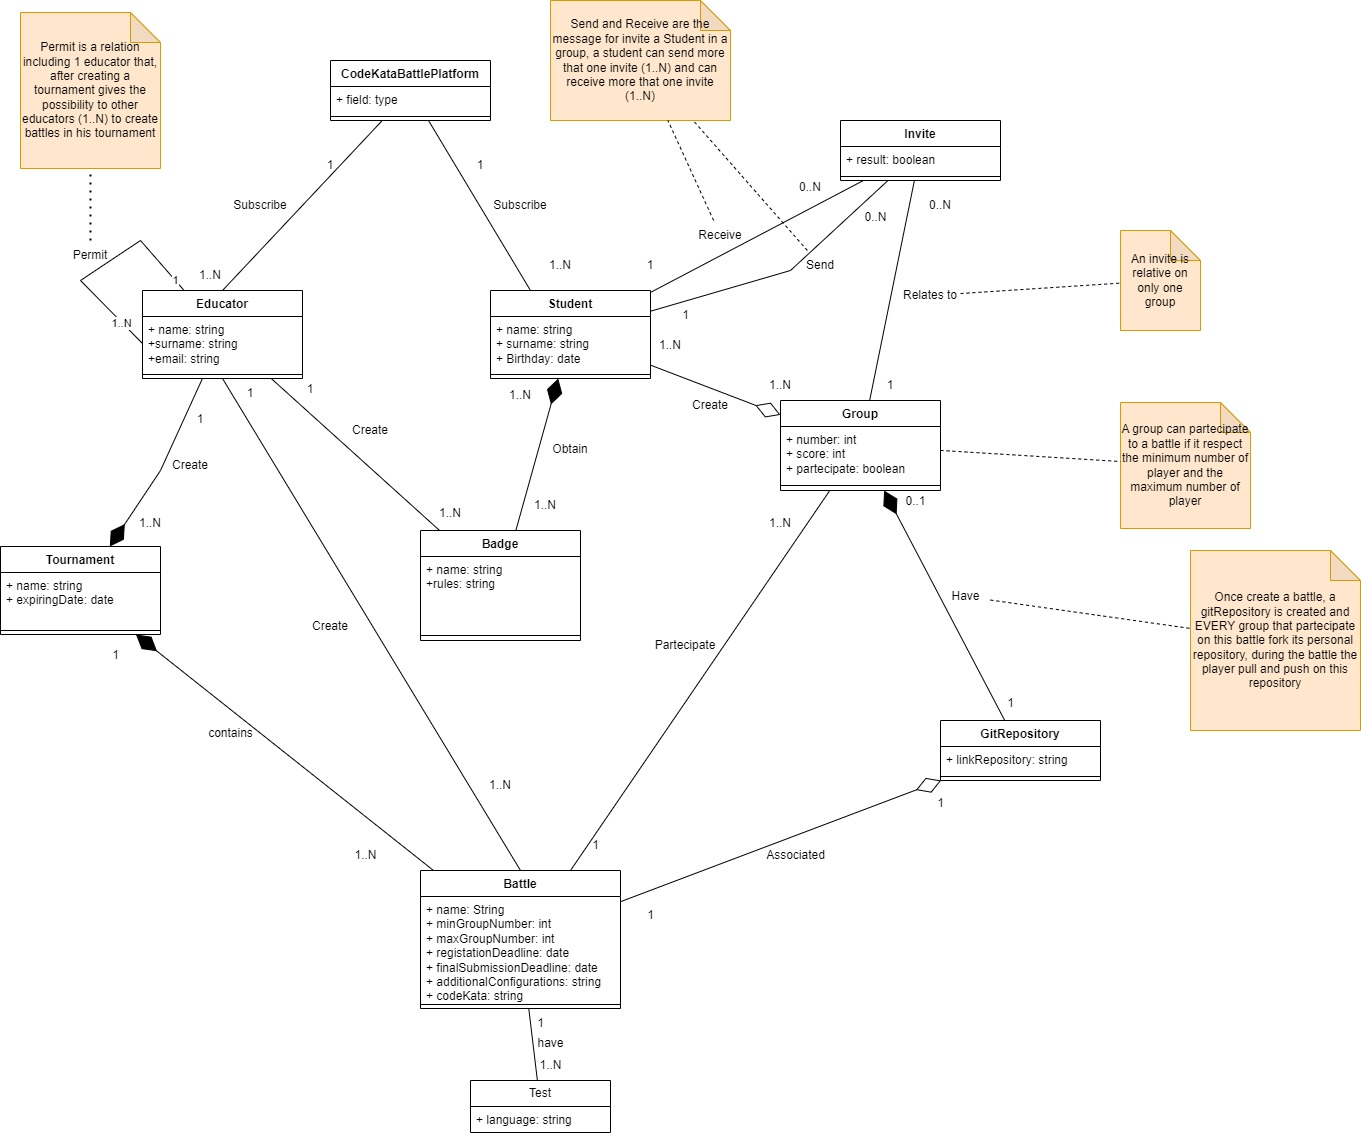
\includegraphics[scale=0.4]{images/ClassDiagram/ClassDiagramFinal.jpg}
            \caption{Class Diagram}
            \label{fig:classDiagram}
        \end{figure}
        
        \newpage
        
\subsection{Product functions}
    \subsubsection{Shared functions}
        \begin{itemize}
            \item \textbf{Sign-up:} Let the user (either students or educators) sign-up to the platform.
            \begin{figure}[H]
                \centering
                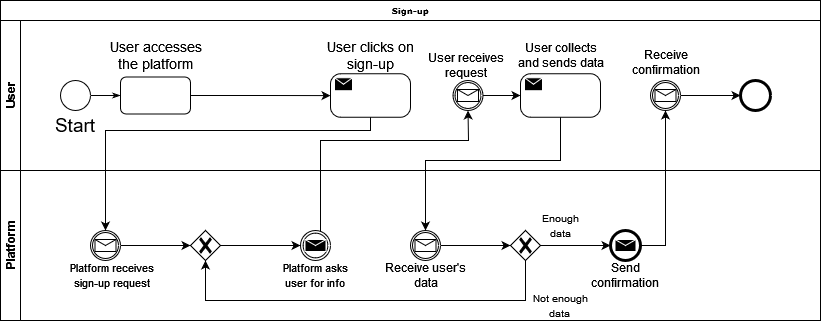
\includegraphics[scale=0.4]{images/BPMN/Sign_up.png}
                \caption{Sign-up BPMN}
                \label{fig:signUpBPMN}
            \end{figure}

            \item \textbf{Visualize student's profile:} Let an user (either a student or an educator) to visualize the profile page of a specific student.
            \begin{figure}[H]
                \centering
                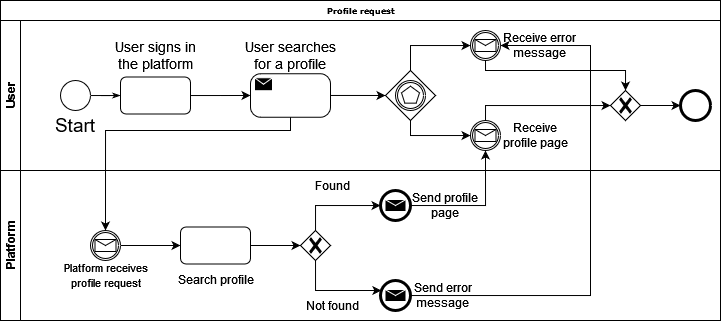
\includegraphics[scale=0.4]{images/BPMN/Profile_request.png}
                \caption{Profile visualization BPMN}
                \label{fig:profileVisualizationBPMN}
            \end{figure}
        \end{itemize}

    \subsubsection{Student functions}
        \begin{itemize}
            \item \textbf{Student subscribes to a tournament:} Let a student search, according to some parameters (most used programming languages, creation date, number of partecipant, etc...) and subscribe to a tournament, after loggin in the platform.
            \begin{figure}[H]
                \centering
                \hspace*{-1.85cm}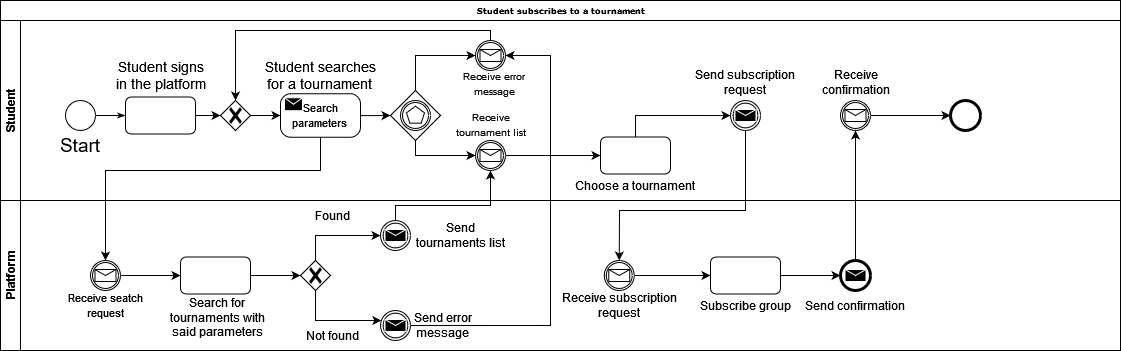
\includegraphics[scale=0.4]{images/BPMN/Tournament_subscription.png}
                \caption{Student's tournament subscription BPMN}
                \label{fig:studTournamentSubBPMN}
            \end{figure}

            \item \textbf{Student join a battle:} Let a student subscribed to a tournament search a battle in it according to some parameters (programming language requested, expiration date, difficulty, etc...) and join it alone or in a group.
            \begin{figure}[H]
                \centering
                \hspace*{-1.85cm}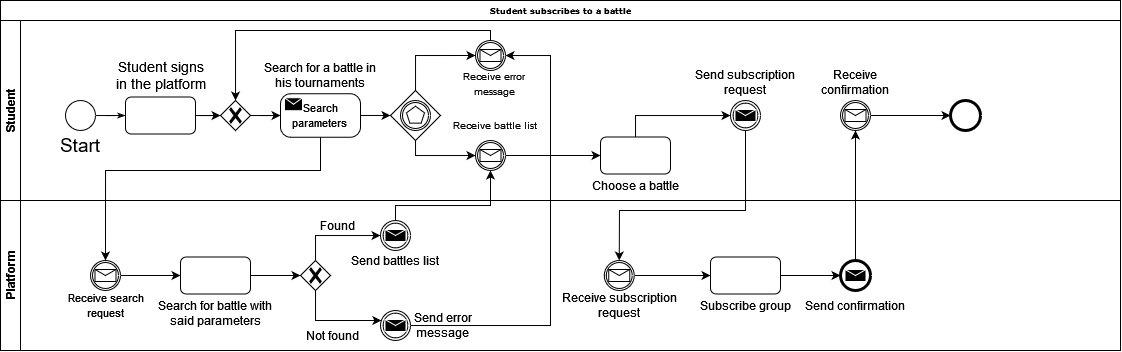
\includegraphics[scale=0.4]{images/BPMN/BattleSubscription.png}
                \caption{Student's battle joining BPMN}
                \label{fig:studBattleJoinBPMN}
            \end{figure}

            \item \textbf{Student gets notified of new events:} Notify the student about new tournaments created, if signed to the platform, and new upcoming battles that take place in tournaments in which he has joined.
            \begin{figure}[H]
                \centering
                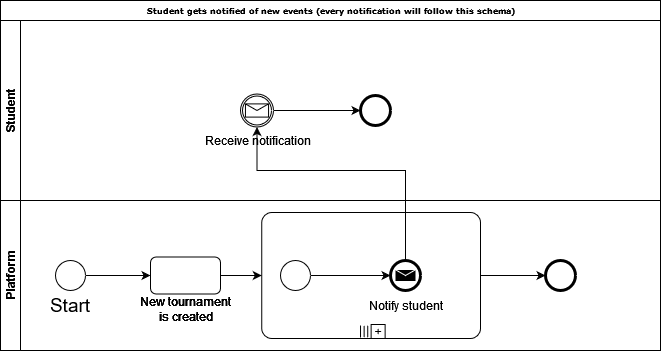
\includegraphics[scale=0.4]{images/BPMN/StudentNotification.png}
                \caption{Student notification BPMN}
                \label{fig:studNotificationBPMN}
            \end{figure}
            
            \item \textbf{Student's solutions get evaluated:} Let a student, who connects to his forked repository on GitHub, upload his solution and evaluate it according to some parameters.
            \begin{figure}[H]
                \centering
                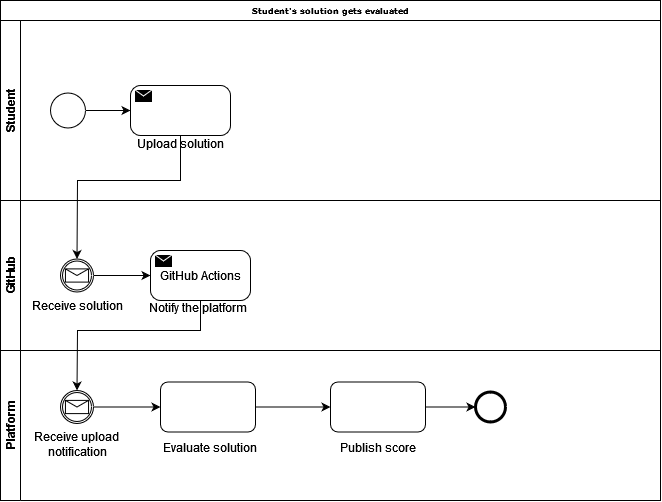
\includegraphics[scale=0.4]{images/BPMN/SolutionEval.png}
                \caption{Student's solutions evaluation BPMN}
                \label{fig:studSolEvalBPMN}
            \end{figure}

            \item \textbf{Student form a group for a battle:} Let a student form a group with other students in order to face a battle, through invite messages.
            \begin{figure}[H]
                \centering
                \hspace*{-1.85cm}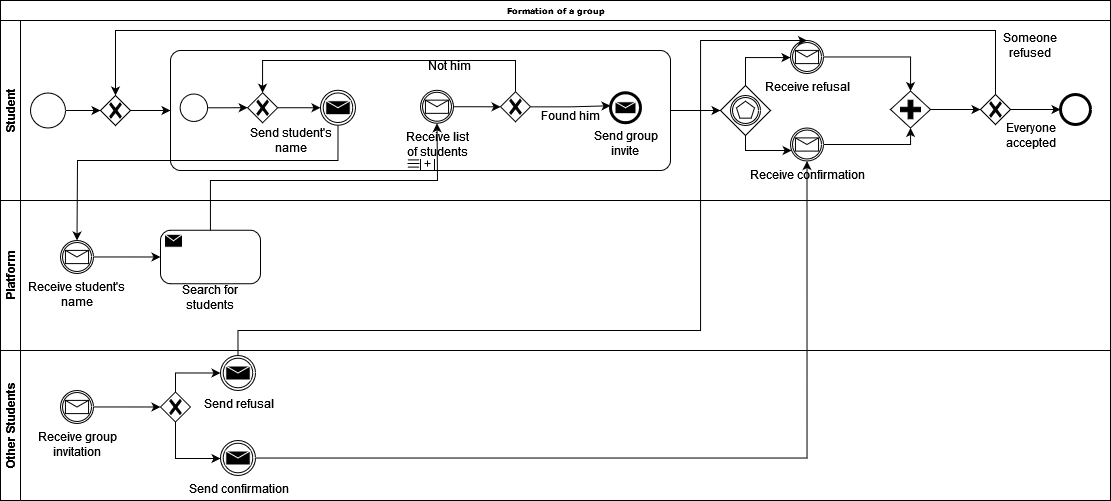
\includegraphics[scale=0.4]{images/BPMN/GroupFormation.png}
                \caption{Formation of a group BPMN}
                \label{fig:groupFormationBPMN}
            \end{figure}
        \end{itemize}

    \subsubsection{Educator functions}
        \begin{itemize}
            \item \textbf{Educator create a tournament:} Let an educator create a new tournament and set its parameters.
            \begin{figure}[H]
                \centering
                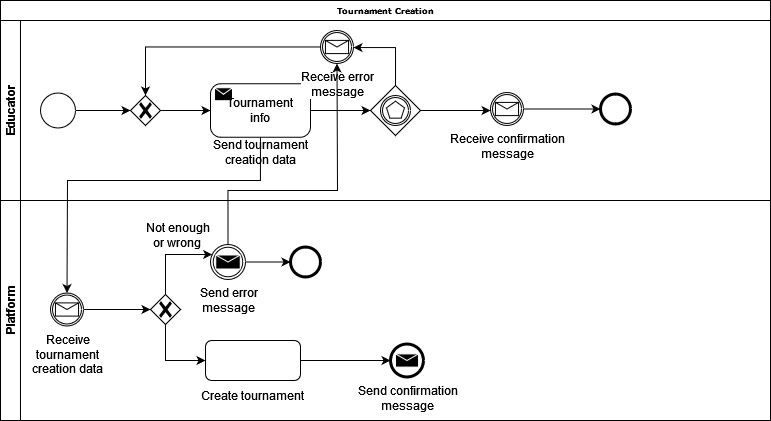
\includegraphics[scale=0.4]{images/BPMN/TournamentCreation.png}
                \caption{Tournament's creation BPMN}
                \label{fig:TournamentCreationBPMN}
            \end{figure}

            \item \textbf{Educator close a tournament:} Let an educator close one of his tournaments whenever he wants.
            \begin{figure}[H]
                \centering
                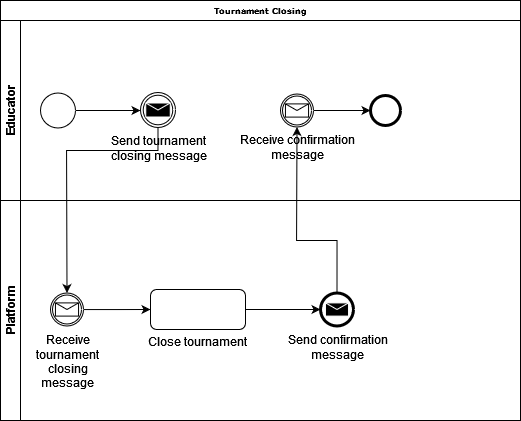
\includegraphics[scale=0.4]{images/BPMN/TournamentClosing.png}
                \caption{Tournament's closing BPMN}
                \label{fig:TournamentClosingBPMN}
            \end{figure}

            \item \textbf{Educator grant access to a tournament:} Give an educator the possibility to grant the access to one of his tournaments to a colleague.
            \begin{figure}[H]
                \centering
                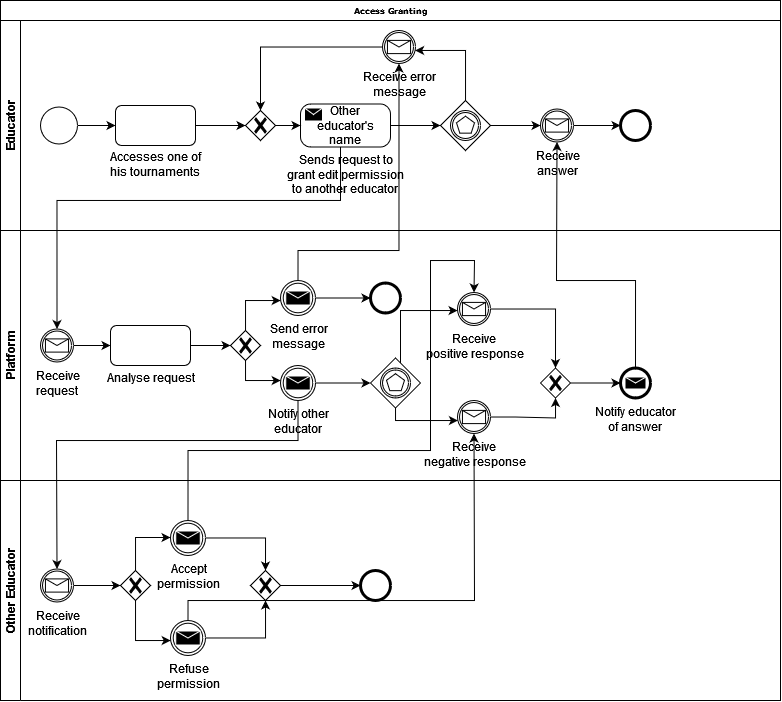
\includegraphics[scale=0.4]{images/BPMN/GrantAccess.png}
                \caption{Grant access to tournament BPMN}
                \label{fig:accessGrantTournamentBPMN}
            \end{figure}

            \item \textbf{Educator creates a battle:} Grant an educator the possibility of creating a battle in tournaments where he has permission to.
            \begin{figure}[H]
                \centering
                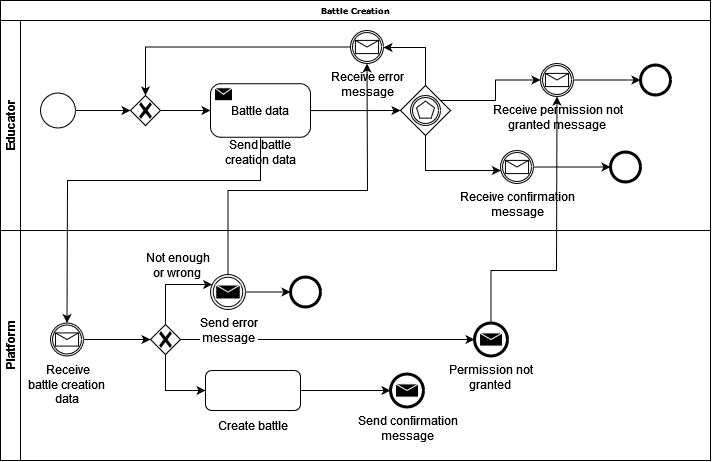
\includegraphics[scale=0.4]{images/BPMN/BattleCreation.png}
                \caption{Create battle BPMN}
                \label{fig:createBattleBPMN}
            \end{figure}

            \item \textbf{Educator notified of battle's end:} Educator gets notified about the end of a battle in one of his tournaments, give him the possibility to manually evaluate the students' solutions.
            \begin{figure}[H]
                \centering
                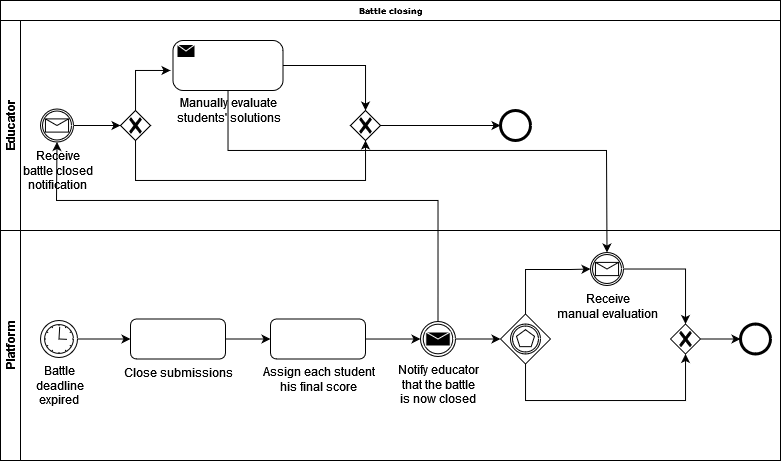
\includegraphics[scale=0.4]{images/BPMN/BattleClosing.png}
                \caption{Ending of a battle BPMN}
                \label{fig:battleEndingBPMN}
            \end{figure}
        \end{itemize}
\subsection{User characteristics}
    \subsection{Assumptions, dependencies and constraints}
        \begin{itemize}
            \item[\textbf{D1:}] Students and educators have access to internet while using the platform
            \item[\textbf{D2:}] Students and educators have their own IT device to connect to the application
            \item[\textbf{D3:}] Students and educators have to be subscribed to the platform in order to use its features
            \item[\textbf{D4:}] Students know how to use GitHub actions
            \item[\textbf{D5:}] Students know how to fork a repository in GitHub
            \item[\textbf{D6:}] A student can join a battle only if subscribed to the tournament in which that battle take place
            \item[\textbf{D7:}] GitHub platform offers reliable services through its API allowing to CKB platform to always get notified when new code is uploaded by students.
            \item[\textbf{D8:}] Educator know how to create new badges, and new rules to obtain them, for the tournaments
            \item[\textbf{D9:}] Time information about registration and submission deadlines for tournaments and battles are always correct.
            \item[\textbf{D10:}] Code written by students can not make the platform crash while testing it.
            \item[\textbf{D11:}] Educators upload ,when creating a battle, some correct, meaningful and faultproof test cases and automation scripts.
            \item[\textbf{D12:}] Students score is always correctly calculated and meaningful.
            \item[\textbf{D13:}] Educators access always access a tournament either in view-only mode, if not invited by the tournament's creator, or in modify-enabled mode if the tournament's creator has granted him the access.
            \textbf{(??? Verificare se potrebbe essere un goal piuttosto che una assumption ???)}
        \end{itemize}

\section{Specific requirements}
\subsection{External interface requirements}
\subsection{Functional requirements}
    \subsubsection{Requirements}
        \subsubsection{Use case diagrams}
            \begin{itemize}
                \item \underline{\large{\textbf{Student}}}
                    \begin{figure}[H]
                        \centering
                        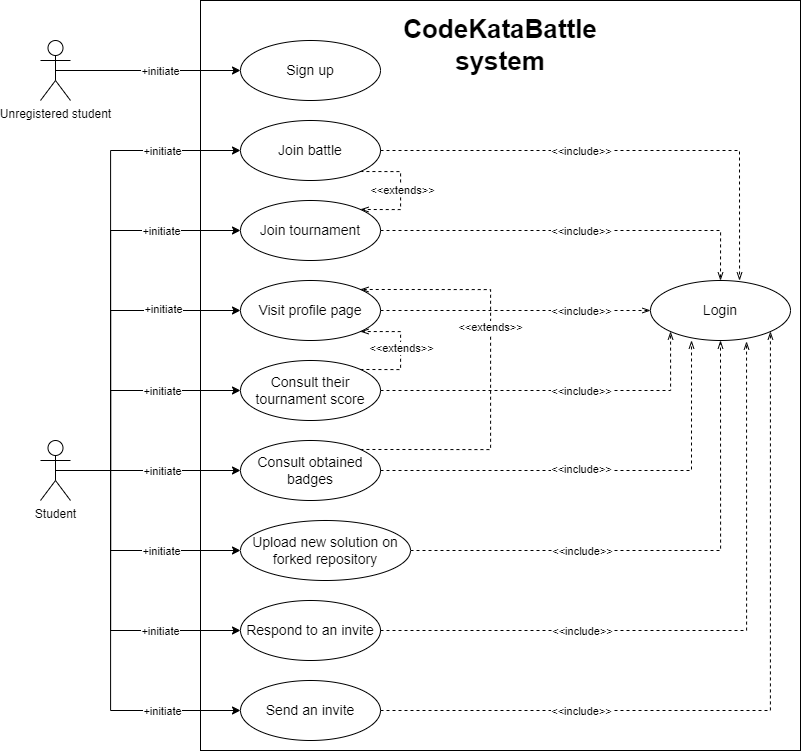
\includegraphics[scale=0.4]{images/3.2.2_UseCaseDiagrams/CaseDiagramStudent.png}
                        \caption{Student use case diagram}
                        \label{fig:studentUseCaseDiagram}
                    \end{figure}
                    
                    N.B: The repository citated in this diagram, on which the student upload their solution, it's not
                    part of the platform. The system, in fact, relies on a third party service (GitHub) to handle the repository.
                    This use case was specified in order to better clarify the tight interaction between the system and the student trought the GitHub service.
                \item \underline{\large{\textbf{Educator}}}
                    \begin{figure}[H]
                        \centering
                        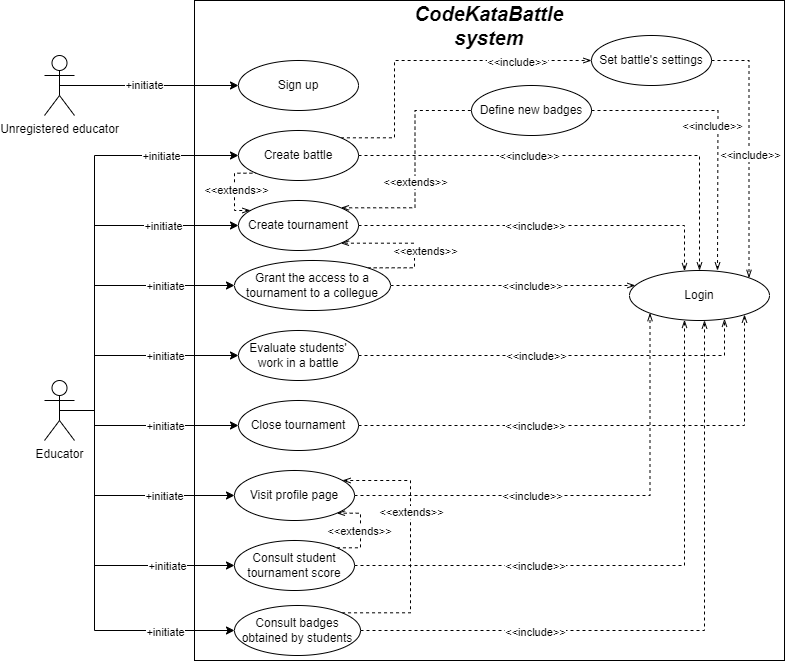
\includegraphics[scale=0.4]{images/3.2.2_UseCaseDiagrams/CaseDiagramEducator}
                        \caption{Educator use case diagram}
                        \label{fig:educatorUseCaseDiagram}
                    \end{figure}
                \item \underline{\large{\textbf{GitHub}}}
                    \begin{figure}[H]
                        \centering
                        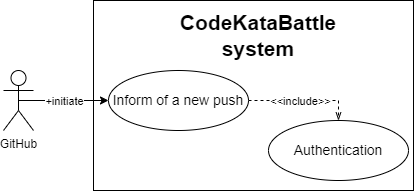
\includegraphics[scale=0.4]{images/3.2.2_UseCaseDiagrams/CaseDiagramGitHub}
                        \caption{GitHub use case diagram}
                        \label{fig:gitHubUseCaseDiagram}
                    \end{figure}
                
            \end{itemize}
        \subsubsection{Use cases w/ sequence diagrams}
            \begin{enumerate}
                \item[\textbf{1.}] \textbf{Student sign up to the platform}

                    \begin{xltabular}{\textwidth}
                        {| >{\raggedright\arraybackslash}g | >{\raggedright\arraybackslash}X |}      
                        \hline
                        \endfirsthead
                        \hline
                        \endhead
                        \endfoot
                        \hline
                        \endlastfoot
                        

                        
                        
                        \textbf{Name} & Student sign up \\
                        \hline
                        \textbf{ID} & UC.1 \\
                        \hline
                        \textbf{Actors} & Unregistered student \\
                        \hline
                        \textbf{Entry condition} & Student want to register to the platform \\
                        \hline
                        \textbf{Flow of events} &    \begin{enumerate}
                                                \item[1.] Student opens CKB platform
                                                \item[2.] Student presses the sign-up button
                                                \item[3.] Student fills the form with all the required informations (name, surname, username
                                                        attended school, email, password, ...), accepts the "Terms \& Conditions".
                                                \item[4.] Student clicks on a button to confirm.
                                                \item[5.] CKB platform validates the personal information inserted by the student.
                                                \item[6.] CBK platform display a confirmation message.
                                                \item[7.] CKB platform send an email notification to the student regarding the registration outcome
                                            \end{enumerate}   \\
                        \hline
                        \textbf{Exit condition} & Student's account is created, and its data are saved into the system\\
                        \hline
                        \textbf{Exceptions} &     \begin{itemize}
                                            \item[4.1] Email already used to register another account, or inexisting.
                                            \item[4.2] Inserted attended school non existings
                                            \item[4.3] Username contains forbidden characters
                                            \item[4.4] Password don't respect security standards 
                                            \begin{itemize}
                                                \item[$\rightarrow$] Unregistered student gets notified of the registration failure throught an 
                                                error message and flow restart from point 3.
                                            \end{itemize} 
                                        \end{itemize}
                        
                    \end{xltabular}
                    
                    
                    \begin{figure}[H]
                        \centering
                        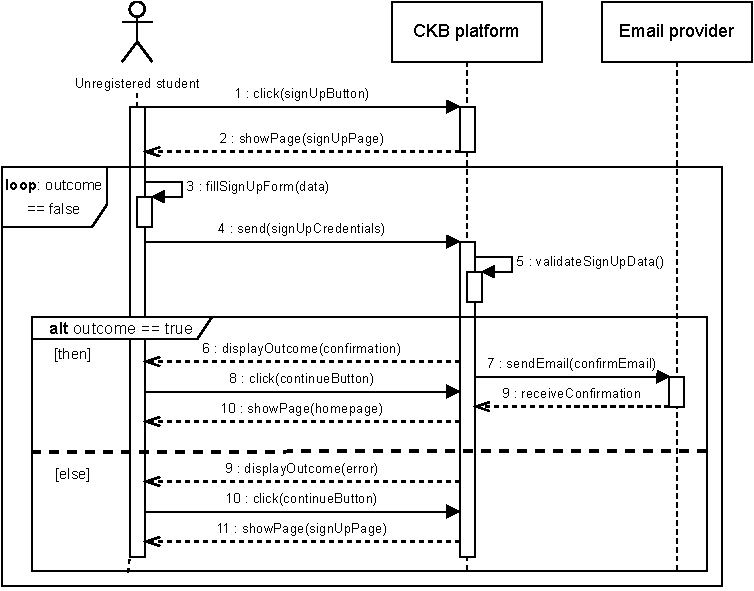
\includegraphics[scale=0.95]{SequenceDiagrams/StudentSignUpSeqDiagram.pdf}
                        \caption{Student sign up sequence diagram}
                        \label{fig:StudentSignUpSeqDiagram}
                    \end{figure}
                    
                
                \item[\textbf{2.}] \textbf{Educator sign up to the platform}
                    \begin{xltabular}{\textwidth}
                        {| >{\raggedright\arraybackslash}g | >{\raggedright\arraybackslash}X |}      
                        \hline
                        \endfirsthead
                        \hline
                        \endhead
                        \endfoot
                        \hline
                        \endlastfoot
                        

                        
                        
                        \textbf{Name} & Educator sign up \\
                        \hline
                        \textbf{ID} & UC.2 \\
                        \hline
                        \textbf{Actors} & Unregistered educator \\
                        \hline
                        \textbf{Entry condition} & Educator want to register to the platform \\
                        \hline
                        \textbf{Flow of events} &    \begin{enumerate}
                                                \item[1.] Educator opens CKB platform
                                                \item[2.] Educator presses the sign-up button
                                                \item[3.] Educator fills the form with all the required informations (name, surname, username
                                                        school in which teaches, istitutional email, password, ...), accepts the "Terms \& Conditions".
                                                \item[4.] Educator clicks on a button to confirm.
                                                \item[5.] CKB platform validates the personal information inserted by the student.
                                                \item[6.] CBK platform display a confirmation message.
                                                \item[7.] CKB platform send an email notification to the educator regarding the registration outcome
                                            \end{enumerate} \\
                        \hline
                        \textbf{Exit condition} & Student's account is created, and its data are saved into the system \\
                        \hline
                        \textbf{Exceptions} &     \begin{itemize}
                                                    \item[4.1] Email already used to register another account, or inexisting.
                                                    \item[4.2] Inserted school's details non correct
                                                    \item[4.3] Username contains forbidden characters
                                                    \item[4.4] Password don't respect security standards 
                                                    \begin{itemize}
                                                        \item[$\rightarrow$] Unregistered educator gets notified of the registration failure throught an error message
                                                        and flow restart from point 3.
                                                    \end{itemize} 
                                                \end{itemize}
                    \end{xltabular}
                    
                    \begin{figure}[H]
                        \centering
                        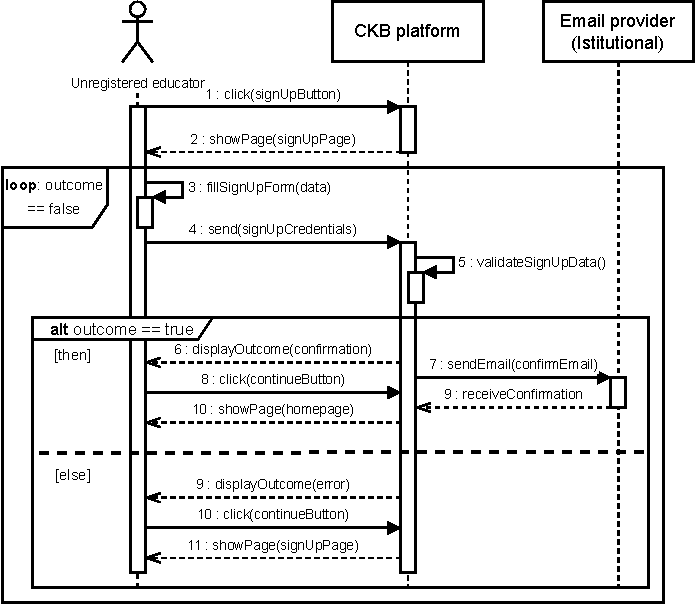
\includegraphics[scale=0.95]{SequenceDiagrams/EducatorSignUpSeqDiagram.pdf}
                        \caption{Educator sign up sequence diagram}
                        \label{fig:EducatorSignUpSeqDiagram}
                    \end{figure}

                    \item[\textbf{3.}] \textbf{Educator creates a new tournament}
                    \begin{xltabular}{\textwidth}
                        {| >{\raggedright\arraybackslash}g | >{\raggedright\arraybackslash}X |}      
                        \hline
                        \endfirsthead
                        \hline
                        \endhead
                        \endfoot
                        \hline
                        \endlastfoot
                        

                        
                        
                        \textbf{Name} & Tournament creation\\
                        \hline
                        \textbf{ID} & UC.3\\
                        \hline
                        \textbf{Actors} & Educator, Student\\
                        \hline
                        \textbf{Entry condition} & Educator has logged in the platform and 
                        want to create a new tournament\\
                        \hline
                        \textbf{Flow of events} &    \begin{enumerate}
                                                        \item[1.] Educator clicks on a "Create tournament" button
                                                        \item[2.] Educator fills a form of the page that has appeared with tournament details,
                                                        such as: its deadline (eventually), allowed programming languages, name, access method and related
                                                        information about how to use it,  etc.
                                                        \item[3.] \textit{$<<$eventually$>>$} Defines new badges for the tournament (see UC.4)
                                                        \item[4.] Educator clicks on a "Confirmation" button.
                                                        \item[5.] CKB platform checks the validity of the informations inserted by the Educator
                                                        \item[6.] CKB platform displays a message that confirms that the tournament
                                                        has been created successfully
                                                    \end{enumerate} \\
                        \hline
                        \textbf{Exit condition} & Tournament is created by saving it's data into the system
                        and the platform sends a notification to all the Students registered to the platform itself.
                        Educator is led back to the riepilogative page of the tournaments created by him. \\
                        \hline
                        \textbf{Exceptions} &    \begin{itemize}
                                                    \item[5.1] Tournament's name contain forbidden characters.
                                                    \item[5.2] Deadline inserted for the tournament is invalid. 
                                                    \item[5.3] Tournament's access method has been configured wrongly.
                                                    \item[5.4] A programming language inserted is not recognized by the platform. 
                                                    \begin{itemize}
                                                        \item[$\rightarrow$] Educator gets notified about the failure of the creation of the tournament
                                                        throught an error message displayed by the platform. The flow restart from point 2.
                                                    \end{itemize} 
                                                \end{itemize}
                    \end{xltabular}
                    
                    \begin{figure}[H]
                        \centering
                        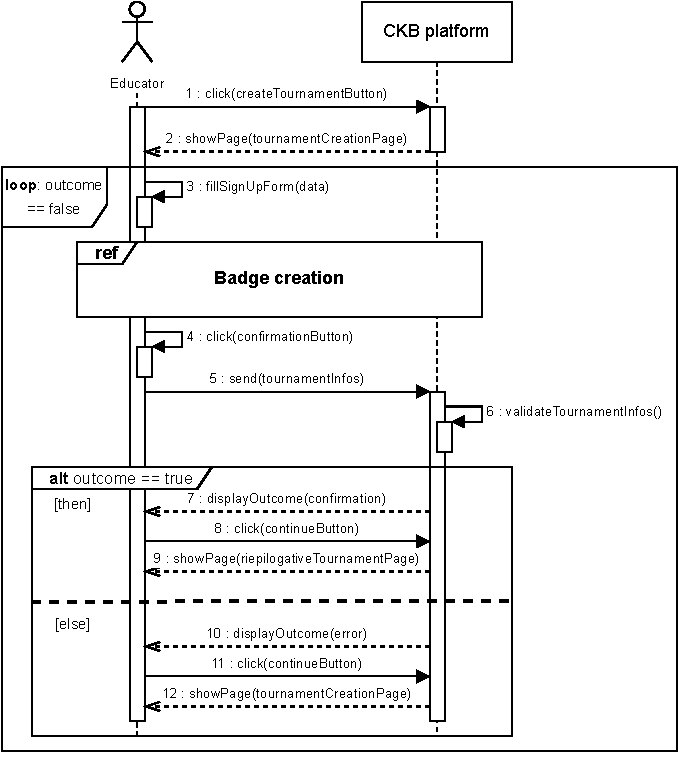
\includegraphics[scale=0.95]{SequenceDiagrams/TournamentCreationSeqDiagram.pdf}
                        \caption{...}
                        \label{fig:TournamentCreationSeqDiagram}
                    \end{figure}

                    \item[\textbf{4.}] \textbf{Educator creates new badges}
                    \begin{xltabular}{\textwidth}
                        {| >{\raggedright\arraybackslash}g | >{\raggedright\arraybackslash}X |}      
                        \hline
                        \endfirsthead
                        \hline
                        \endhead
                        \endfoot
                        \hline
                        \endlastfoot
                        

                        
                        
                        \textbf{Name} & Badges creation\\
                        \hline
                        \textbf{ID} & UC.4\\
                        \hline
                        \textbf{Actors} & Educator\\
                        \hline
                        \textbf{Entry condition} & Educator has logged in the platform, he's creating a new tournament and want to
                        define new badges for that tournament\\
                        \hline
                        \textbf{Flow of events} &    \begin{enumerate}
                                                        \item[1.] Educator clicks on the "Create badge" button on the tournament
                                                        creation page.
                                                        \item[2.] On the new page that appeared, the Educator defines badge's
                                                        characteristics, such as: its name, value, icon, rules to obtain it, ...
                                                        \item[3.] Educator clicks on a button in order to confirm its choices.
                                                        \item[4.] CKB platform checks if all the badge informations are well defined
                                                        \item[5.] CKB platform displays a message that confirm the successfull creation
                                                        of a new badge, and that the badge has been added to the tournament.
                                                    \end{enumerate} \\
                        \hline
                        \textbf{Exit condition} & Badge is created, its data are saved and associated to the
                        tournament which is being created by the Educator and Educator is led back to the 
                        create tournament page. \\
                        \hline
                        \textbf{Exceptions} &    \begin{itemize}
                                                    \item[4.1] Badge's name contain forbidden characters
                                                    \item[4.2] The image uploaded as icon image it's too big or have an unsupported format.
                                                    \item[4.3] Badge's rules are not well defined.   
                                                    \item[4.4] Some badge's features has been left empty  
                                                    \begin{itemize}
                                                        \item[$\rightarrow$] Educator gets notified about the failure of the badge creation
                                                        process throught an error message displayed by the platform. Flow restart from point 2.
                                                    \end{itemize} 
                                                \end{itemize}
                    \end{xltabular}
                    
                    \begin{figure}[H]
                        \centering
                        %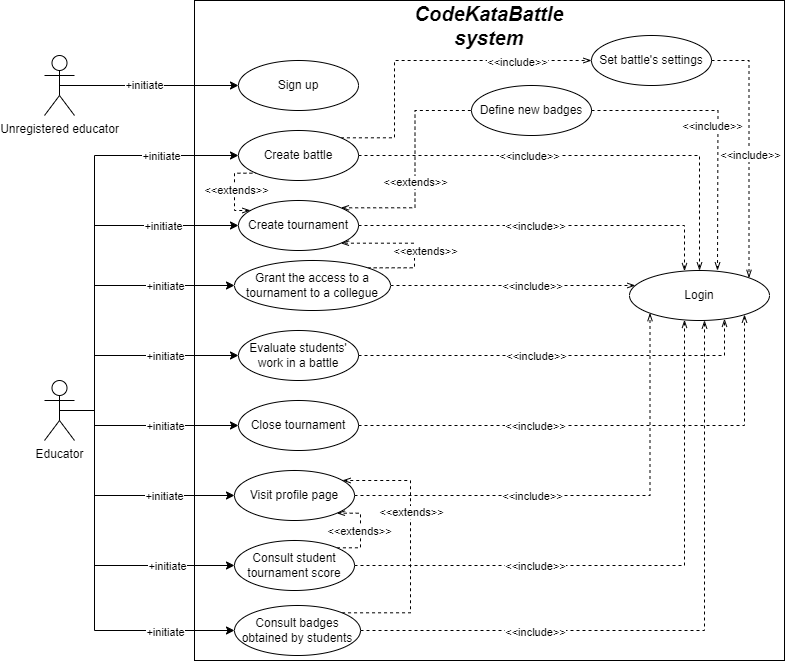
\includegraphics[scale=0.4]{images/3.2.2_UseCaseDiagrams/CaseDiagramEducator}
                        \caption{...}
                        \label{fig:BadgesCreationSeqDiagram}
                    \end{figure}

                    \item[\textbf{5.}] \textbf{Educator delete a badge}
                    \begin{xltabular}{\textwidth}
                        {| >{\raggedright\arraybackslash}g | >{\raggedright\arraybackslash}X |}      
                        \hline
                        \endfirsthead
                        \hline
                        \endhead
                        \endfoot
                        \hline
                        \endlastfoot
                        

                        
                        
                        \textbf{Name} & Deletion \& update of a badge\\
                        \hline
                        \textbf{ID} & UC.5\\
                        \hline
                        \textbf{Actors} & Educator\\
                        \hline
                        \textbf{Entry condition} & Educator has logged in the platform, has started the creation of a new
                        tournament in which has already created at least 1 badge and want to delete and/or update one of them\\
                        \hline
                        \textbf{Flow of events} &    \begin{enumerate}
                                                        \item[1.] Educator clicks on a update button related to the badge and 
                                                        present on the tournament creation page. 
                                                        \item[2.] CKB platform show a modifiable form, filled with the 
                                                        badge's data which the Educator want to modify.
                                                        \item[3.] Educator proceeds to modify the badge's data
                                                        \item[4.] CKB platform tries to validate the new data
                                                        \item[5.] Update is confirmed with the display of a message by the CKB platform. 
                                                        \item[6.] Educator clicks on a delete button related to 
                                                        the badge and present on the tournament creation page. 
                                                        \item[7.] CKB platform show a message requiring confirmation
                                                        for the Deletion
                                                        \item[8.] Educator presses a confirmation button
                                                        \item[9.] CKB platform delete the badge and bring the Educator 
                                                        to the previous page.
                                                    \end{enumerate} \\
                        \hline
                        \textbf{Exit condition} & Deleted badges are removed from the tournament, and their data are removed
                        from the system. The modifications of the updated ones are committed to the system. The Educator
                        is led back to the tournament creation page. \\
                        \hline
                        \textbf{Exceptions} &    \begin{itemize}
                                                    \item[4.1] Badge's updated name contain forbidden characters
                                                    \item[4.2] The new image uploaded as icon, it's too big or have an unsupported format.
                                                    \item[4.3] New Badge's rules are not well defined.
                                                    \item[4.4] Some badge's features has been left empty 
                                                    \begin{itemize}
                                                        \item[$\rightarrow$] Badge it's not updated, Educator it's led to
                                                        the tournament creation page (point 1.)
                                                    \end{itemize}
                                                    \item[6.1] Educator presses the cancel button 
                                                    \begin{itemize}
                                                        \item[$\rightarrow$] Delete procedure is stopped, and the Educator
                                                        it's led back to the tournament creation page (point 6.).
                                                    \end{itemize} 

                                                \end{itemize}
                    \end{xltabular}
                    
                    \begin{figure}[H]
                        \centering
                        %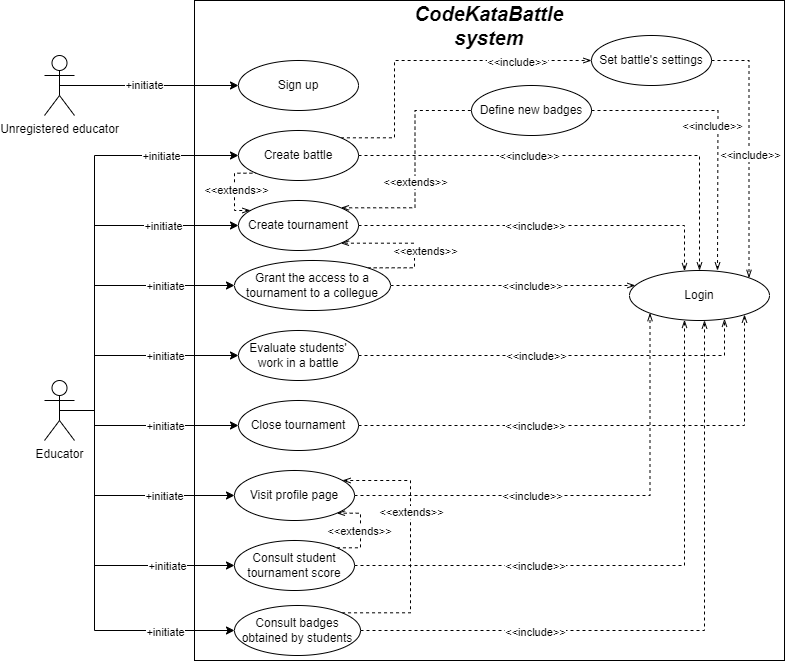
\includegraphics[scale=0.4]{images/3.2.2_UseCaseDiagrams/CaseDiagramEducator}
                        \caption{...}
                        \label{fig:DeletionUpdateBadgesSeqDiagram}
                    \end{figure}

                    \item[\textbf{6.}] \textbf{Educator creates a new battle}
                    \begin{xltabular}{\textwidth}
                        {| >{\raggedright\arraybackslash}g | >{\raggedright\arraybackslash}X |}      
                        \hline
                        \endfirsthead
                        \hline
                        \endhead
                        \endfoot
                        \hline
                        \endlastfoot
                        

                        
                        
                        \textbf{Name} & Battle creation\\
                        \hline
                        \textbf{ID} & UC.6\\
                        \hline
                        \textbf{Actors} & Educator\\
                        \hline
                        \textbf{Entry condition} & Educator has logged in the platform, has created at least 1 tournament
                        and want to add a battle in a specific tournament \\
                        \hline
                        \textbf{Flow of events} &    \begin{enumerate}
                                                        \item[1.] Educator open the page related to a specific tournament
                                                        which has created.
                                                        \item[2.] Educator clicks on a button used to create a new battle.
                                                        \item[3.] Educator fills the form shown by the platform with informations
                                                        related to the battle that he want to create (name, programming languages
                                                        allowed, maximum and minimum number of students for each partecipating 
                                                        group, registration and submission deadlines, ...)
                                                        \item[4.] Educator clicks on a button to confirm.
                                                        \item[5.] CKB platform validates the battle characteristics
                                                        \item[6.] CKB platform display a confirmation message of the successfull
                                                        creation of the battle.
                                                    \end{enumerate} \\
                        \hline
                        \textbf{Exit condition} & New battle, with characteristics specified by the Educator,
                         is created within the tournament chosen by the Educator itself. Educator it's then led to the riepilogative
                         page of the battles within the tournament.
                         \\
                        \hline
                        \textbf{Exceptions} &    \begin{itemize}
                                                    \item[3.1] Battle's name contain forbidden characters
                                                    \item[3.2] A programming language inserted it's not included in the tournament
                                                    allowed programming languages.
                                                    \item[3.3] The specified number of minimum or maximum students for each group
                                                    it's beyond upper and/or lower limits imposed by the platform
                                                    \item[3.4] Registration deadline inserted for the battle it's not valid or
                                                    bigger than the submission one.
                                                    \item[3.5] Submission deadline inserted for the battle it's not valid or 
                                                    smaller than the registration one.
                                                    \begin{itemize}
                                                        \item[$\rightarrow$] Educator gets notified about battle creation failure
                                                        by the platform throught an error message. The flow restart from point 3.
                                                    \end{itemize} 
                                                \end{itemize}
                    \end{xltabular}
                    
                    \begin{figure}[H]
                        \centering
                        %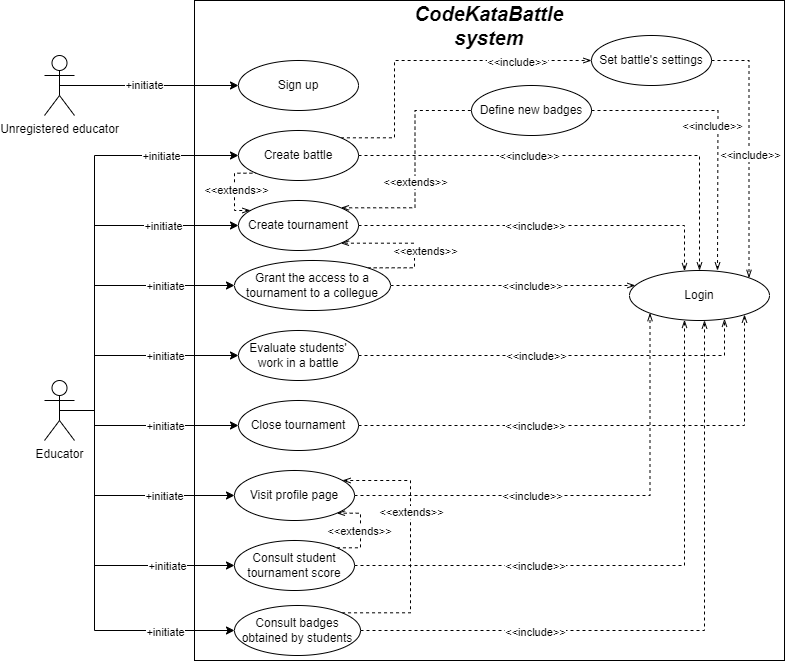
\includegraphics[scale=0.4]{images/3.2.2_UseCaseDiagrams/CaseDiagramEducator}
                        \caption{...}
                        \label{fig:BattleCreationSeqDiagram}
                    \end{figure}
            \end{enumerate}
        \subsubsection{Traceability matrix}
\subsection{Performance requirements}
\subsection{Design constraints}
\subsection{Software system attributes}

\section{Formal analysis using Alloy}

\section{Effort spent}

\section{References}


\end{document}
